\spacing{1.25}
\section{Rayos Cósmicos}
Los rayos cósmicos (RC) son partículas cargadas aceleradas a altas energías que se propagan por el espacio y llegan a la atmósfera terrestre. Un $90\%$ de estas partículas son protones, un $9\%$ núcleos de helio y el resto son electrones, núcleos más pesados y antipartículas. La mayoría de RC son relativistas; su espectro de energías está entre $\sim 10^9$ y $\sim 10^{20}$ eV, y sigue una ley de potencias. Actualmente se tiene conocimiento de fuentes de RC de origen galáctico y extragaláctico \cite{Gaisser1990}. A continuación se describen algunos aspectos del desarrollo histórico de la investigación sobre los RC.
	
	\subsection{Descubrimiento y naturaleza de los RC}
	En el año 1900 se realizaban experimentos para estudiar la ionización causada por elementos radiactivos, en estos se observó que el aire contenía algún tipo de radiación que también era capaz de ionizar. A partir de esto se inició la búsqueda del origen de dicha radiación. Se repitieron los experimentos a alturas de $300$ a $1300$ m, esperando que si la fuente de la radiación fuese la corteza terrestre, ésta disminuiría con la altura. En 1911-1912, el austriaco Victor Hess realizó experimentos en globo a alturas de hasta $5200$ m, con los que concluyó que la radiación debía originarse fuera de la Tierra y que, comparando mediciones de día y de noche, no provenía del sol. Victor Hess es considerado el descubridor de los rayos cósmicos \cite{Extremas}.\\
	
	Posteriormente se inició la búsqueda de la naturaleza de estas partículas, siendo el candidato más popular los rayos gamma. En 1927 Jacob Clay observó una disminución de la radiación en bajas latitudes. Esto fue explicado en 1932 por Arthur Compton como la acción del campo magnético de la Tierra sobre los RC, llevando a la conclusión de que la mayor parte de las partículas en cuestión debían tener carga eléctrica, y estudiando los efectos geomagnéticos este-oeste se dedujo que casi todas las cargas eran positivas. Finalizando la década de 1940, experimentos de detección directa realizados por Schein establecieron que aproximadamente el $99\%$ de los RC son protones, núcleos de Helio y núcleos más pesados y que sólo el $1\%$ son electrones, positrones y rayos gamma \cite{Dorman2004}.

	\subsection{Producción de RC}		
	En la figura \ref{fig:espectro} se muestra el espectro observado de RC, el cual está bien representado por una ley de potencias:
	\begin{align}
	\dv{N}{E}=E^{-(\gamma+1)}.
	\end{align}	
	El índice $\gamma$ tiene un valor aproximadamente constante de $2.7$ con dos ligeros cambios: uno a $\sim 10^{16}$ eV, conocido como la \textit{rodilla}, y el otro a $\sim 10^{19}$ eV conocido como el \textit{tobillo} \cite{Extremas}. El espectro se extiende desde  $\sim 10^9$ hasta $\sim 10^{20}$ eV.
	
	\begin{figure}[h]
	\centering	
	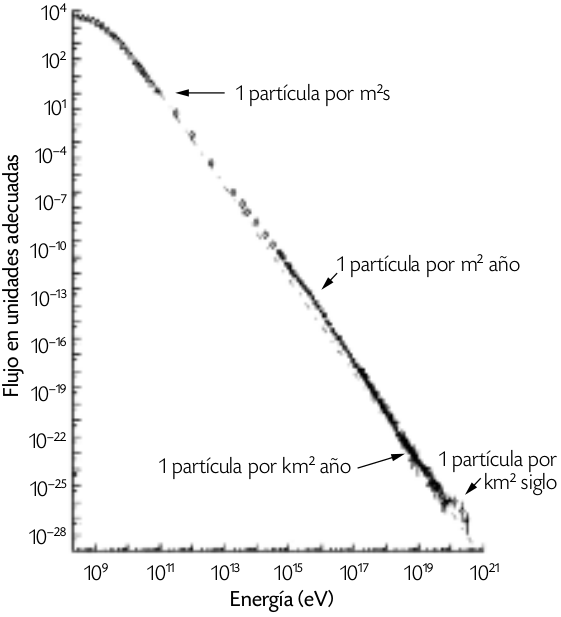
\includegraphics[width=0.5\textwidth]{Figuras/espectro_RC} 
	\caption{Intensidad del flujo de rayos cósmicos en función de su energía. Éste está bien representado por una ley de potencias $E^{-2.7}$. (Tomada de \cite{Poderosas})}
	\label{fig:espectro}
	\end{figure}	

	Por tanto, debe haber un mecanismo capaz de acelerar partículas a tales energías y que reproduzca la forma del espectro observado. En 1949, Fermi propuso un mecanismo en el que las partículas podían ganar energía en colisiones estocásticas en regiones del espacio donde existiesen campos magnéticos turbulentos, como las ondas de choque resultado de un colapso gravitacional, por ejemplo. Se considera que una partícula de prueba tiene un incremento de energía proporcional a la misma $\Delta E = \xi E$ en cada colisión, luego de $n$ colisiones la energía de la partícula será \cite{Gaisser1990}
	\begin{align}
	E_n = E_0 \qty(1+\xi)^n,
	\end{align}
donde $E_0$ es la energía con la que entra al proceso de aceleración. Tomando en cuenta la probabilidad $P_{esc}$ de que la partícula escape de la región de aceleracón, la proporción de partículas que se aceleran a energías mayores a un valor $E$ es
	\begin{align}
	N(\geq E) \propto \frac{1}{P_{esc}}\qty(\frac{E}{E_0})^{-\gamma},
	\end{align}
	con $\gamma = -\ln(1-P_{esc})/\ln(1+\xi) \approx P_{esc}/\xi$, de manera que este mecanismo efectivamente reproduce la ley de potencias que caracteriza al espectro de RC. \\
	
	El mecanismo de Fermi se describe en dos situaciones físicas: nubes de plasma magnetizadas (aceleración de Fermi de segundo orden) y frentes de onda de choque (aceleración de Fermi de primer orden). En la aceleración de segundo orden se considera una partícula que entra a la nube con cierta velocidad, donde cambia su dirección de modo aleatorio por interacciones con el campo magnético turbulento en el interior, mediante este proceso se tiene $\xi=(4/3) \beta^2$, donde $\beta= V/c$ es la velocidad de la nube; en la aceleración de primer orden se considera que la partícula atraviesa la onda de choque e interactúa con el campo magnético del gas que éste va dejando detrás (\textit{downstream}), en este caso $\xi=(4/3) \beta$, donde $\beta= V/c$ se refiere la velocidad del gas detrás del choque respecto al gas delante del choque (\textit{upstream}).
	
	\subsection{Fuentes de RC}
	Luego de establecer cómo pueden acelerarse las partículas, se buscaron objetos astronómicos que cumplan las condiciones necesarias para que el proceso se lleve a cabo. Para que el proceso sea eficaz, la partícula debe estar contenida en una región de radio $R$, tal que se cumpla la siguiente relación \cite{DeAngelis2015}:	
	\begin{align}
	E[\text{PeV}] \simeq B[\mu\text{G}]\times R[\text{pc}].
	\end{align}
	Ésta es llamada relación de Hillas, ilustrada en la figura \ref{fig:Hillas}, en la que también pueden observarse los potenciales aceleradores. Como fuentes de RC de origen galáctico pueden mencionarse las estrellas de neutrones de rápida rotación (púlsares) y los remanentes de supernova, mientras que en el caso extragaláctico se consideran los núcleos galácticos activos y los destellos de rayos gamma.
	
	\begin{figure}[h]
	\centering	
	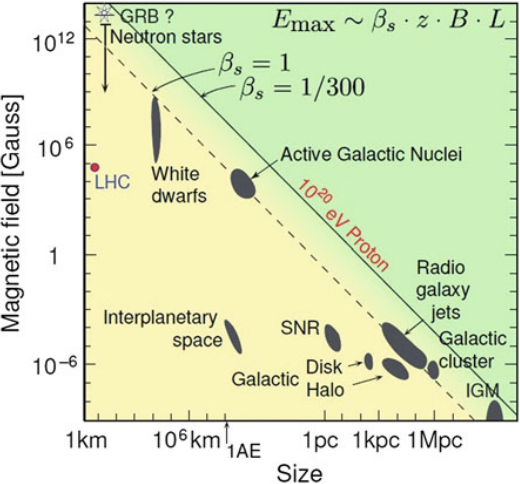
\includegraphics[width=0.5\textwidth]{Figuras/Hillas_Relation} 
	\caption{La gráfica de Hillas representa las potenciales fuentes de rayos cósmicos según la intensidad de su campo magnético y su tamaño. (Tomada de \cite{DeAngelis2015})}
	\label{fig:Hillas}
	\end{figure}	

	\subsection{Propagación de RC}
	La presencia de campos magnéticos en el espacio limita la posibilidad de estudiar las fuentes de RC a través de ellos. Los RC llegan a la Tierra isotrópicamente; llegan de todas direcciones con la misma frecuencia, lo que sugiere una trayectoria casi aleatoria desde la fuente hacia la Tierra. Dentro de la galaxia las partículas pueden sufrir varios procesos: difusión en campos magnéticos, convección por vientos galácticos, pérdidas o ganancias de energía, colisiones nucleares con gas interestelar y decaimientos. Para describir la propagación de RC debe resolverse la ecuación de transporte \cite{Gaisser1990}:
	\begin{align}
	\pdv{\mathcal{N}}{t} &= \nabla \cdot \qty(D_i \nabla \mathcal{N}_i)-\pdv{E} \qty[b_i(E)\mathcal{N}_i(E)]-\nabla \cdot u \mathcal{N}_i(E) \nonumber \\
	&+ Q_i(E,t) - p_i \mathcal{N}_i + \frac{v \rho}{m} \sum_{k \geq i}\int \frac{\dd \sigma_{i,k}\qty(E,E')}{\dd E}\mathcal{N}_k(E')\dd E',
	\end{align}
	que contempla los procesos mencionados para calcular la densidad de partículas con energías entre $E$ y $E+\dd E$. Los seis términos de la ecuación representan, respectivamente: la difusión, ganancias de energía, convección, la inyección de partículas, pérdida de partículas por colisiones o decaimientos, cascadas de decaimientos o fragmentación nuclear. 

\section{Interacciones de los RC}
	\subsection{Interacciones electromagnéticas}
	Las partículas cargadas en general interactúan con átomos; estas pueden ionizarlos, excitarlos o producir fotones. Para electrones y positrones a altas energías es relevante la radiación de frenado o \textit{bremsstrahlung}, en la cual partículas cargadas emiten radiación al ser deflectadas por el campo eléctrico de los átomos en un medio. En este proceso, la fracción de energía que la partícula pierde puede describirse por \cite{DeAngelis2015}:
	\begin{align}
	\frac{1}{E} \dv{E}{x} \simeq -\frac{1}{X_0},
	\end{align}
	donde $X_0$ es la longitud de radiación que es dependiente del medio.\\
	
	Por otro lado, los fotones interactúan con un medio principalmente mediante efecto fotoeléctrico (emisión de un electrón de un material que ha absorbido un fotón), dispersión de Compton (transferencia de energía de un fotón hacia un electrón mediante una colisión) y producción de pares electrón-positrón. Este último proceso siendo el más relevante a altas energías; al interactuar con el campo eléctrico de un núcleo, el fotón tiene cierta probabilidad de formar un par $e^{-}-e^{+}$, con una longitud de interacción:
	\begin{align}
	\lambda \simeq \frac{9}{7} X_0.
	\end{align}	
 	\\ 
	Los fotones también puede sufrir otros procesos como dispersión de Rayleigh, que puede tener importancia para el transporte de la luz a través de la atmósfera, o interacciones fotonucleares (excitación de núcleos) que se dan a energías alrededor de $10$ MeV.
	
	\subsection{Interacciones hadrónicas}
	Los RC primarios están mayoritariamente conformados por hadrones, como lo son los protones y núcleos. Los hadrones se describen mediante el modelo de quarks \cite{DeAngelis2015}, partículas que interactúan mediante la interacción nuclear fuerte y que, según observaciones, no existen de manera aislada sino en estados ligados de dos o tres quarks. Este tipo de modelos se estudian desde la \textit{cromodinámica cuántica} (QCD por sus siglas en inglés), donde se propone el concepto de \textit{color} como la carga que origina las interacciones fuertes, y el de \textit{gluón} como la partículas mediadora. \\
		
	\begin{wrapfigure}{r}{0.3\textwidth}
	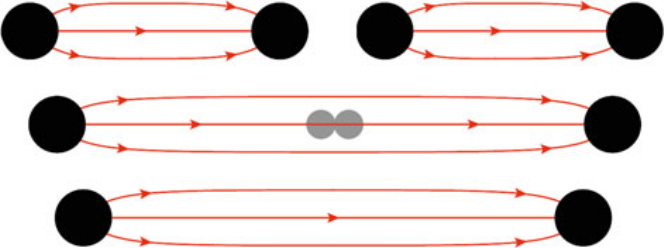
\includegraphics[width=0.3\textwidth]{Figuras/string_frag} 
	\caption{De abajo hacia arriba; fragmentación de una cuerda creando un nuevo par de quarks en el campo de color. (Tomado de \cite{DeAngelis2015})}
	\label{fig:string}
	\end{wrapfigure}		
	
	Para describir las interacciones hadrónicas se necesitan modelos fenomenológicos apoyados en QCD. Un modelo usado comúnmente es el modelo de cuerdas de Lund (o \textit{string model}) \cite{FragModels}; cuando los hadrones interactúan se forma un campo de color (cuerda) entre pares quark-antiquark, la energía potencial en dicha cuerda aumenta hasta fragmentarse y formar otros quarks que a su vez pueden formar hadrones, como se ilustra en la figura \ref{fig:string}. También suele utilizarse el modelo de \textit{minijet}, para tomar en cuenta la multiplicidad de partículas producidas. \\

	Actualmente existen varios generadores Monte Carlo de eventos hadrónicos; describen este tipo de interacciones basándose en diferentes modelos para ciertos aspectos de la interacción y en datos de colisionadores de partículas. Ejemplos de estos son SIBYLL \cite{Sibyll}, QGSJET \cite{qgsjet} y EPOS \cite{EPOS}, que están especializados en interacciones de altas energías. 
	

\section{Chubascos atmosféricos}
	Un chubasco atmosférico (español para \textit{Air Shower}) es una cascada de partículas generada por la interacción de un rayo cósmico primario en la alta atmósfera. Antes de profundizar en cómo se desarrollan estas cascadas, conviene describir brevemente las principales características de la atmósfera.
	
	\subsection{Atmósfera terrestre}
	La capa de aire que rodea la Tierra se extiende hasta una altura  mayor a $100$ km. Según el modelo \textit{US Standard Atmosphere}, la atmósfera está compuesta principalmente por N$_2$ ($78$ \%), O$_2$ ($21$ \%) y Ar ($0.9$ \%). Acorde al mismo modelo, la densidad del aire es función de la altura:
	\begin{align}
	\rho(h)=\rho_0 e^-\frac{h}{h_a},
	\end{align}
	donde $\rho_0 = 1.22\times 10^{-3}$ g/cm$^3$ y $h_a = 8.2$ km. Sin embargo, en el estudio de los chubascos atmosféricos es más frecuente utilizar el concepto de \textit{profundidad} en lugar de la altura. La profundidad $X$ indica la cantidad de materia que atraviesa una partícula al moverse de un punto a otro. Esta se relaciona con la densidad mediante:
	\begin{align}
	X = \int_h^{\infty} \rho (h) \dd h.
	\end{align}

	\subsection{Desarrollo de un chubasco atmosférico}	
	Los chubascos atmosféricos se desarrollan de forma compleja como una combinación de cascadas electromagnéticas y producción de partículas por interacciones hadrónicas \cite{Matthews2005}. A grandes rasgos, una interacción hadrónica entre el rayo cósmico primario y un núcleo de la atmósfera produce partículas secundarias: una partícula principal (con la mayor parte de la energía inicial) que puede iniciar otro chubasco, y un gran número de mesones, principalmente piones cargados ($\pi^{\pm}$) y neutros ($\pi^0$).\\

	La parte electromagnética del chubasco es generada por los piones neutros al decaer en fotones ($\pi^0 \rightarrow \gamma \gamma$), esta cascada consiste en producción de pares ($\gamma\rightarrow e^+ e^-$) y bremsstrahlung ($e^{\pm} \rightarrow e^{\pm}\gamma$). Por su parte, los piones cargados pueden volver a interactuar hadrónicamente mientras tengan suficiente energía, luego de eso decaerán en neutrinos y muones ($\pi^{-} \rightarrow \mu^- \bar{\nu}_{\mu}$, $\pi^{+} \rightarrow \mu^+ \nu_{\mu} $). El desarrollo de un chubasco se ilustra en la figura \ref{fig:airshower}.\\
				
	\begin{figure}[h]
	\centering
	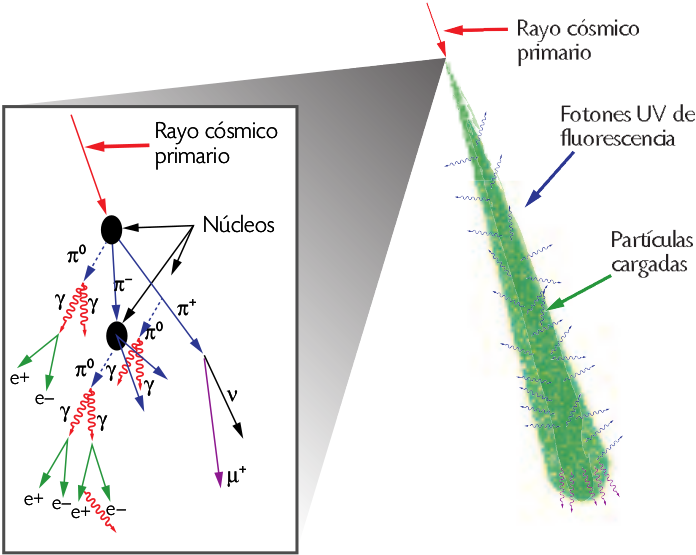
\includegraphics[width=0.6\textwidth]{Figuras/air_shower} 
	\caption{Esquema de la formación y desarrollo de un chubasco atmosférico. Se observa la componente hadrónica y la electromagnética. (Tomada de \cite{Poderosas})}
	\label{fig:airshower}
	\end{figure}	

	La propagación de partículas (nucleones en particular) a través de la atmósfera, puede describirse con la ecuación de cascada:
	\begin{align}
	\dv{N(E,X)}{X} = -\frac{N(E,X)}{\lambda_N(E)} + \int_E^{\infty}\frac{N(E',X)}{\lambda_N(E)} F_{NN}(E,E') \frac{\dd E'}{E},
	\end{align}
	donde $N(E,X) \dd E$ es el flujo de nucleones a una profundidad $X$ en la atmósfera con energías entre $E$ y $E+\dd E$, $\lambda_N$ es la \textit{longitud de interacción} del nucleón en el aire y $F_{NN}$ es la sección eficaz para la colisión de un nucleón incidente de energía $E'$ con un núcleo del aire, produciendo otro nucleón con energía $E$. Para generalizar al caso de la propagación de los múltiples hadrones producidos, se considera un grupo de ecuaciones acopladas \cite{Gaisser1990}:
	\begin{align}
	\dv{N_i(E,X)}{X} = -\qty(\frac{1}{\lambda_i}+\frac{1}{d_i}) N_i(E,X) + \sum_i \int \frac{F_{ij}(E_i,E_j)}{E_i} \frac{N_j(E_j)}{\lambda_j} \dd{E_j}.
	\end{align}
	
	\subsection{Métodos de observación}
	Existen distintos tipos de experimentos para observar chubascos atmosféricos, la técnica utilizada depende principalmente de la energía del rayo cósmico incidente; a energías $>50$ TeV pueden detectarse partículas secundarias directamente a nivel del suelo, mientras que a energías $\sim$TeV pueden observarse recolectando la radiación producida en las interacciones de las partículas. \\
	
	Los experimentos pueden ser de \textit{radiación de Cherenkov}, que detectan radiación producida por una partícula cargada que se mueve a través de un medio más rápido que la velocidad de la luz en ese medio; y de \textit{fluorescencia}, que colectan la luz emitida por las moléculas de nitrógeno excitadas en el chubasco, este método permite reconstruir el desarrollo longitudinal del mismo. Existen también observatorios híbridos, como el \textit{Telescope Array} (TA) y el \textit{Pierre Auger Observatory} (PAO); estos utilizan la técnica de fluorescencia para observar el desarrollo del chubasco y además detectan partículas de alta energía que alcanzan el nivel del suelo.
	
\section{Estado del conocimiento}
En la actualidad, los RC de ultraalta energía (UHECR, $E > 10^{18}$ eV) siguen considerándose un enigma en términos de su composición y origen. Debido a su bajo flujo, éstos se estudian indirectamente a partir de mediciones de los chubascos atmosféricos que producen. Experimentos como TA y PAO miden observables de los chubascos como $X_{max}$, $X_{max}^{\mu}$ y $N_{\mu}$, magnitudes que son sensibles a la energía y la masa de la partícula primaria, y por tanto pueden aportar al espectro de RC y dar información sobre la composicion del flujo de los UHECR. Con ayuda de programas de simulación de chubascos atmosféricos, como CORSIKA, CONEX y AIRES, se ha progresado en esta dirección.\\

\begin{figure}[h]
\centering
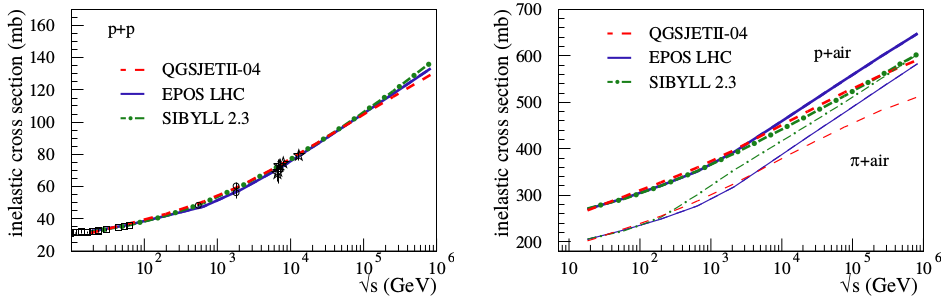
\includegraphics[width=0.95\textwidth]{Figuras/Pierog2018} 
\caption{Sección eficaz inelástica para interacciones p-p (izquierda) e interacciones p-aire y $\pi$-aire (derecha) calculadas con tres modelos hadrónicos \cite{Pierog2018}.}
\label{fig:cross_sections}
\end{figure}	

Dichos programas utilizan modelos de interacciones hadrónicas, que son mayoritariamente fenomenológicos, consecuentemente el estudio de los UHECR está estrechamente vinculado con la investigación experimental de colisiones hadrónicas de alta energía en aceleradores de partículas. Los parámetros de las interacciones que afectan el desarrollo de los chubascos atmosféricos son la sección eficaz, la multiplicidad y la elasticidad; se han comparado diferentes modelos (Sibyll 2.3, EPOS LHC y QGSJETII-04) observando que coinciden muy bien para interacciones $p-p$, pero difieren para interacciones $p-A$ y $\pi-A$ \cite{Pierog2018}. \\

La interpretación de las mediciones observacionales para dilucidar la composición de los UHECR es todavía un problema, esto es debido particularmente a que los modelos de interacciones hadrónicas aún difieren entre sí y ninguno de ellos puede describir a cabalidad los datos. La interpretación de los datos del TA se inclina por una composición de núcleos ligeros \cite{TAcomposition}, mientras que datos del PAO indican que la composición se vuelve más pesada a mayores energías. Sobre esto último, se realizó un ajuste simulando chubascos iniciados por una mezcla de partículas primarias (p, He, N y Fe) que resultó en buena concordancia con los datos de $X_{max}$ \cite{PAOcomposition}. Sin embargo, la interpretación está sujeta al modelo utilizado para las simulaciones.\\

\begin{figure}[h]
\centering
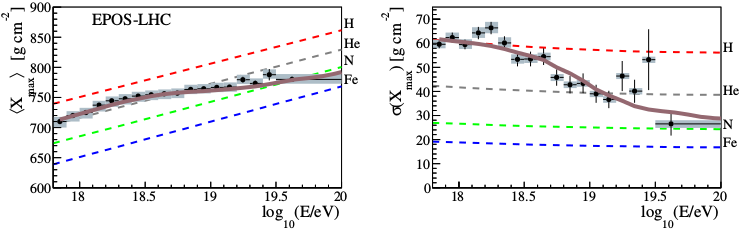
\includegraphics[width=0.95\textwidth]{Figuras/Xmax_PAO} 
\caption{$X_{max}$ promedio (izquierda) y desviación estándar (derecha) asumiendo una composición mixta (línea sólida) \cite{PAOcomposition}.}
\label{fig:Xmax}
\end{figure}	

Se han considerado cambios en el tratamiento de ciertos aspectos físicos en los modelos \cite{Ostapchenko2019} con los cuales se mejora la simulación de $X_{max}$ y $X_{max}^{\mu}$ comparándolo con los datos de PAO. También se ha presentado una discusión sobre $N_{\mu}$, ya que el número de muones predicho por simulaciones es significativamente menor que el observado; se puso a prueba la hipótesis de una composición mixta de los UHECR estudiando su impacto sobre $N_{\mu}$, reduciendo la diferencia entre las simulaciones y las observaciones a una constante \cite{Sciutto2019}.

\begin{figure}[h]
\centering
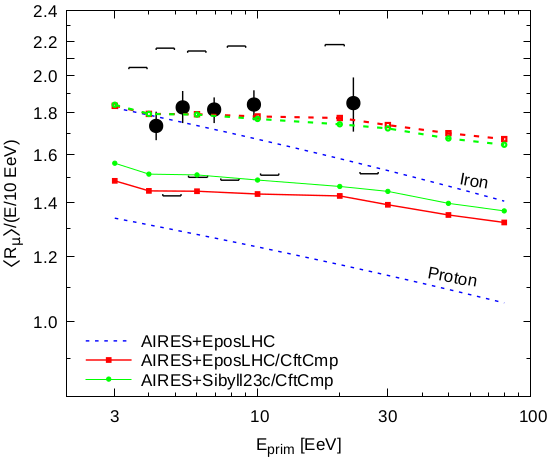
\includegraphics[width=0.7\textwidth]{Figuras/Nmu_Sciutto} 
\caption{Las líneas sólidas verde y roja corresponden a la estimación del número de muones utilizando el sistema AIRES con diferentes modelos hadrónicos. Se observa que al desplazarlas una constante éstas tienen buena concordarcia con los datos experimentales (círculos negros) \cite{Sciutto2019}.}
\label{fig:Nmu}
\end{figure}	

\singlespace


